\documentclass{beamer}
\usepackage[utf8]{inputenc}
\usepackage[english]{babel}
\usepackage{helvet}
\usepackage[T1]{fontenc}
\usepackage{textcomp}
\usepackage[inline]{asymptote}
\usepackage{slide_helper}
\usepackage{multirow}
\usepackage{tikz}
\usepackage{subfigure}
\usepackage{fp}
\usepackage{cancel}
\usetikzlibrary{shapes.geometric, arrows}
\usepackage{pgfplots}
\pgfplotsset{compat=1.5} 
\usepgfplotslibrary{statistics}
\usetikzlibrary{external}
\tikzexternalize%

\title[MA205 - Section 3.4]{Random Variables}

\DeclareSymbolFont{extraup}{U}{zavm}{m}{n}
\DeclareMathSymbol{\varheart}{\mathalpha}{extraup}{86}
\DeclareMathSymbol{\vardiamond}{\mathalpha}{extraup}{87}
\DeclareMathSymbol{\varclub}{\mathalpha}{extraup}{84} 
\DeclareMathSymbol{\varspade}{\mathalpha}{extraup}{85}

\newcommand{\suitheart}[1][]{{\color{red}\text{#1}\varheart}}
\newcommand{\suitspade}[1][]{{\color{black}\text{#1}\spadesuit}}
\newcommand{\suitdiamond}[1][]{{\color{red}\text{#1}\vardiamond}}
\newcommand{\suitclub}[1][]{{\color{black}\text{#1}\varclub}}
\newcommand{\card}[2]{{#1{\color{black}\text{#2}}}}

\newcommand{\prob}[1]{P\left({#1}\right)}
\newcommand{\jointprob}[3]{\prob{{#1}~\text{#2}~{#3}}}
\newcommand{\condprob}[2]{\prob{{#1}~|~{#2}}}
\newcommand{\comb}[2]{_{#1}C_{#2}}

\newcommand\encircle[1]{%
  \tikz[baseline=(X.base)]  % chktex 36 chktex 1
    \node (X) [draw, shape=circle, inner sep=0, fill=yellow!10] {\strut #1};} % chktex 36 chktex 1

\begin{document}
\begin{frame}
\titlepage
\end{frame}

\begin{frame}
\begin{example}\label{bookstore}
\vspace{-2mm}%beamer bug: extra space is added when a label is used, so this is to make this slide and the next look the same
Two books are assigned for a course: 
\begin{itemize}
\item A textbook, which costs \$137.
\item The accompanying study guide, which costs \$33.
\end{itemize}\pause

The university bookstore determined:
\begin{itemize}
\item 20\% of enrolled students do not buy either book.
\item 55\% of enrolled students only buy the textbook.
\item 25\% of the enrolled students buy both books.
\end{itemize}\pause

\question{How many books should be expected to sell if 100 students enrolled?}\pause
\answer{We expect about 25 students will buy none, 55 will buy just the textbook, and 25 will buy both. A total of $ 1\cdot 55 + 2\cdot 25 = 105$ books.}\pause

\vspace{2mm}
\question{How much revenue should be expected to be made?}\pause
\answer{$\$0\cdot 25 + \$137\cdot 55 + (\$137+\$33)\cdot 25\pause = \$7,535 + \$4,250 \pause = \$11,785$}\pause

\vspace{2mm}
\question{What is the average revenue per student?}\pause
\answer{$\$11,785 \div 100~\text{students} \pause = \$117.85$ per student.}
\end{example}
\end{frame}

\begin{frame}
\begin{definition}
A \textbf{random variable} is a random process or variable that has a numerical value, determined by chance, for each outcome.
\end{definition}\pause

\begin{note}
Often capital letters such as $X$, $Y$, or $Z$ are used for random variables.

\vspace{1mm}
Corresponding lower case letters are used for the possible outcomes.
\end{note}\pause

\begin{example}
Consider tossing a coin: We could get either a heads or a tails.\pause

\vspace{1mm}
If we let $X$ be the number of tails we get in a single flip, then the two possible outcomes are: $x_1=0$ and $x_2=1$.\pause

\vspace{2mm}
The probability distribution is:
\begin{center}
\begin{tabular}{lccc}\hline
$i$ & 1 & 2 & Total \\\hline
$x_i$ & 0 & 1 & -- \\
$\prob{X=x_i}$ & 0.50 & 0.50 & 1.00 \\\hline
\end{tabular}
\end{center}
\end{example}
\end{frame}

\begin{frame}
\begin{example}\label{bookstore random variable}
\vspace{-2mm}%beamer bug: extra space is added when a label is used, so this is to make this slide and the next look the same
If we let $X$ be the amount a student spends in Example~\ref{bookstore}, then the probability distribution is:
\begin{center}
\begin{tabular}{lcccc}\hline
$i$ & 1 & 2 & 3 & Total \\\hline
$x_i$ & \$0 & \$137 & \$170 & -- \\
$\prob{X=x_i}$ & 0.20 & 0.55 & 0.25 & 1.00\\\hline
\end{tabular}
\end{center}
\end{example}\pause 

\begin{definition}
A \textbf{discrete random variable} has a collection of values that is finite or countable.
\end{definition}\pause

\begin{definition}
A \textbf{continuous random variable} has infinitely many values, and the collection of values is not countable.
\end{definition}\pause

\begin{note}
The random variable in Example~\ref{bookstore random variable} is a discrete random variable.
\end{note}
\end{frame}

\begin{frame}
\begin{example}
Let's consider tossing two coins, with the following random variable:

\vspace{-3mm}
\begin{equation*}
X=\text{number of heads when two coins are tossed}
\end{equation*}\pause

\vspace{-5mm}
\question{Is $X$ is a discrete or continuous random variable?}\pause
\answer{$X$ is discrete since the number of heads can be 0, 1, or 2.}\pause

\vspace{2mm}
The probability distribution is:
\begin{center}
\begin{tabular}{lcccc}\hline
$i$ & 1 & 2 & 3 & Total \\\hline
$x_i$ & 0 & 1 & 2 & -- \\
$\prob{X=x_i}$ & 0.25 & 0.50 & 0.25 & 1.00\\\hline
\end{tabular}
\end{center}\pause
\end{example}
\end{frame}

\begin{frame}
\begin{example}
Hiring managers were asked to identify the biggest mistakes that job applicants make during an interview. 

\vspace{2mm}
Consider the following table:
\begin{center}
\begin{tabular}{llc}\hline
$i$ & $x_i$ & $\prob{X=x_i}$ \\\hline
1 & \text{Inappropriate attire} & 0.50 \\
2 & \text{Being late} & 0.44 \\
3 & \text{Lack of Eye Contact} & 0.33 \\
4 & \text{Checking phone or texting} & 0.30 \\\hline
\multicolumn{2}{r}{Total} & 1.57\\\hline
\end{tabular}
\end{center}
\question{Is $X$ and random variable?}\pause
\answer{%
\begin{enumerate}
\item The outcomes are not numerical, they are categorical.\pause
\item $\sum \prob{X=x_i}=1.57\neq 1$\pause
\end{enumerate}
So, we see that $X$ is not a random variable.}
\end{example}
\end{frame}

\begin{frame}
\begin{definition}
The average outcome of $X$ is called the \textbf{expected value} of $X$.
\end{definition}\pause

\begin{example}
In Example~\ref{bookstore} the average revenue, \$117.85 per student, is the expected value for the bookstore's revenue.

\begin{center}
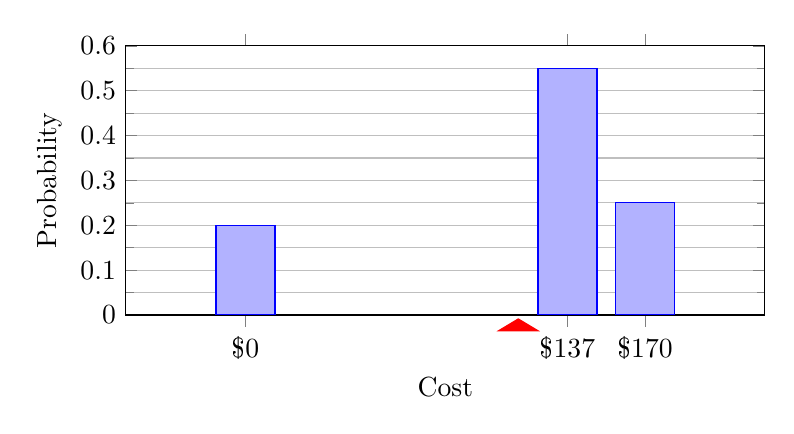
\begin{tikzpicture}
\FPeval\expectedx{clip(4.987)} %chktex 36
\FPeval\expectedy{clip(-0.05)} %chktex 36

\FPeval\expectedwidth{clip(0.25)} %chktex 36
\FPeval\expectedheight{clip(0.15)} %chktex 36

\FPeval\aptx{clip(\expectedx-\expectedwidth)} %chktex 36
\FPeval\apty{clip(\expectedy-\expectedheight)} %chktex 36

\FPeval\bptx{clip(\expectedx)} %chktex 36
\FPeval\bpty{clip(\expectedy)} %chktex 36

\FPeval\cptx{clip(\expectedx+\expectedwidth)} %chktex 36
\FPeval\cpty{clip(\expectedy-\expectedheight)} %chktex 36

\begin{axis}[
height=5.0cm,
width=0.8\textwidth,
enlarge x limits=0.3,
ymajorgrids=true,
minor y tick num=1,
yminorgrids=true,
ylabel={Probability},
xlabel={\variable{Cost}},
bar width=0.75cm,
%symbolic x coords={\$0, \$137, \$170},
ybar,
ymin=0,
ymax=0.6,
ytick={0,0.1,...,1},
xtick=data,
xticklabel style={/pgf/number format/.cd,fixed,precision=0},
xticklabel=\$\pgfmathprintnumber{\tick},
]
\addplot+
coordinates
{
(0, 0.2)
(137, 0.55)
(170, 0.25)
};
%\draw[red] (axis cs: 117.58,0) -- (axis cs: 117.58, 0.1);
\end{axis}
\filldraw[red] (\aptx,\apty) -- (\bptx, \bpty) -- (\cptx,\cpty) -- cycle;
\end{tikzpicture}
\end{center}
\end{example}
\end{frame}

\begin{frame}
\begin{block}{Expected Value Of A Discrete Random Variable}
If $X$ takes outcomes $x_1$, \ldots, $x_k$ with probabilities $\prob{X=x_1}$, \ldots, $\prob{X=x_k}$, the expected value of $X$ is:
\begin{equation*}
\begin{aligned}
E(X) &= x_1\cdot\prob{X=x_1} + x_2\cdot\prob{X=x_2} + \cdots + x_k\cdot\prob{X=x_k} \\
&= \sum_{i=1}^{k} x_i\cdot\prob{X=x_i}
\end{aligned}
\end{equation*}\pause
\end{block}

\begin{note}
The Greek letter $\mu$ is sometimes used in place of $E(X)$.
\end{note}
\end{frame}

\begin{frame}
\begin{example}
In the casino game Roulette, a wheel with 38 numbered spaces is spun. There are 18 red spaces, 18 black spaces, and 2 green spaces. \pause

\vspace{1mm}
In one possible bet, the players bet \$1 on a single number. If that number is spun on the wheel, then they receive \$36. Otherwise, they lose their \$1.\pause

\vspace{1mm}
If $X$ is the net winnings, then the probability distribution is:
\begin{center}
\begin{tabular}{lccc} \hline
$i$ & 1 & 2 & Total \\\hline
$x_i$ & \$35 & -\$1 & -- \\
$\prob{X=x_i}$ & $\dfrac{1}{38}$ & $\dfrac{37}{38}$ & 1\\[2mm]\hline
\end{tabular}
\end{center}\pause

The expected value of $X$ is:

\vspace{-2mm}
\begin{equation*}
\begin{aligned}
E(X) &= x_1\cdot\prob{X=x_1} + x_2\cdot\prob{X=x_2} + x_3\cdot\prob{X=x_3} \\\pause
&= \$35\cdot\dfrac{1}{38} + -\$1\cdot\dfrac{37}{38} \pause = \$0.9211 - \$0.9737 \pause \approx -\$0.053
\end{aligned}
\end{equation*}\pause

\vspace{-3mm}
On \emph{average}, the player will lose 5.3 cents per bet.
\end{example}
\end{frame}

\begin{frame}
\begin{note}
Pick back up here. The following slides need to be editied
\end{note}
\end{frame}

\begin{frame}
\begin{example}
Suppose an individual has a 0.242\% risk of dying during the next year. An insurance company charges \$275 for a life-insurance policy that pays \$100,000 death benefit. What is the expected value for the person buying the insurance?\pause

\vspace{2mm}
The probabilities and values for the two outcomes are:
\begin{center}
\begin{tabular}{|r|r|} \hline
Value & Probability \\ \hline
\$100,000-\$275 = \$99,725 & 0.00242 \\ \hline
-\$275 & 1-0.00242 = 0.99758 \\ \hline
\end{tabular}
\end{center}\pause
The expected value is $\$99,725\cdot 0.00242 -\$275\cdot0.99758 = -\$33$.
\end{example}\pause
\begin{note}
It makes sense that a insurance policy would have a negative expected value, otherwise the insurance company couldn't stay in business.

\vspace{2mm}
The benefit for the consumer is the security that the policy provides.
\end{note}
\end{frame}

\begin{frame}
\begin{example}
A company estimates that 0.7\% of their products will fail after the original warranty period but within 2 years of the purchase, with a replacement cost of \$350. If they offer a 2 year extended warranty for \$48, what is the company's expected value?\pause

\vspace{2mm}
The probabilities and values for the two outcomes are:
\begin{center}
\begin{tabular}{|r|r|} \hline
Value & Probability \\ \hline
-\$350 + \$48 = -\$302 & 0.007 \\ \hline
\$48 & 1-0.007 = 0.993 \\ \hline
\end{tabular}
\end{center}\pause
The expected value is $-\$302\cdot 0.007 + \$48\cdot0.993 = \$45.55$.

\vspace{2mm}
The company makes, on average, \$45.55 on each extended warranty.
\end{example}\pause

\begin{note}
The expected value for the consumer may be different. The consumer is likely to pay the more to repair or replace the item out of warranty.\\ (The company pays manufacturing cost, consumer has to pay retail cost.)
\end{note}
\end{frame}
\end{document}
